% ch08-systems.tex -- Traps, memory-mapped IO, and a running machine
\chapter{Traps, memory-mapped IO, and a program that talks to the world}
\label{ch:systems08}

The core built over chapters~5--7 computes correctly, but it is a
closed box: it can neither call for help when something goes wrong
nor emit a single observable byte. This chapter opens two doors at
once. A minimal trap mechanism --- \texttt{ecall} to enter a handler,
\texttt{mret} to return --- gives the machine its first taste of
exception handling. A memory-mapped UART gives it a voice. By the
end, one testbench run shows a program compute \(6\times 7\), print
\texttt{42} on a serial wire, trap into a handler that prints
\texttt{K}, return, print \texttt{!}, and park --- all on real
Verilog, all bytes decoded off the simulated wire.

\begin{rulebox}[After this chapter you can]
You will be able to run one Verilog simulation of a pipelined RV32I
core and say, from the printed log alone, which of its four output
bytes came from the main program and which from the trap handler. You
will be able to write the two instructions that print a byte through a
memory-mapped UART, decode a serial frame by hand, and work out how
long a software delay must be so that a byte is not lost.
\end{rulebox}

\begin{rulebox}[Before you start]
Think of a restaurant kitchen. The core you built in chapters~5--7 is a
kitchen that cooks very well but has no door to the dining room and no
bell that a waiter can ring. This chapter adds the bell (a \emph{trap})
and the serving window (a \emph{UART}). Here is what you need to
remember from earlier, in plain words.
\emph{Pipeline} (chapter~6): the core works like an assembly line with
five stations, IF (fetch the instruction), ID (decode it), EX (compute),
MEM (touch memory) and WB (write the result back), and each instruction
moves one station per clock cycle.
\emph{Hazards} (chapter~7): when two instructions in the line depend on
each other, the hardware either \emph{forwards} a result early, or
\emph{stalls} (freezes the front of the line for a cycle), or
\emph{flushes} (throws away instructions that were fetched from the
wrong place). We will use flush again today.
\emph{Instructions} (chapter~3): \texttt{sw rs2, off(rs1)} writes the
register \texttt{rs2} to the memory address \texttt{rs1+off}, and
\texttt{lui} puts a constant into the upper 20 bits of a register.
\emph{Serial transmitter} (Book~5, electronics, chapter~13, section
``UART: talking to the outside world''): a shift register that puts one
bit on a single wire per tick. If that is hazy, do not worry; the frame
diagram in section~\ref{sec:uart08} redraws everything you need.
\end{rulebox}

\begin{rulebox}[Think like this]
When a machine does something you cannot see, ask: \emph{what is the
smallest observation that would prove it?} A counter of wire edges is a
weak observation. A receiver that reads the bytes back is a strong one.
This chapter climbs from the first to the second.
\end{rulebox}

\section{Two small additions, one big change of character}
\label{sec:doors08}

Why does a processor need these at all? Picture a clerk who only ever
does sums on paper. She is useful, but she cannot say what she found
(no output), and she cannot be interrupted when something goes wrong
(no way to ask for help). Both problems are solved by giving the
hardware a small, fixed set of ways to talk to the world. Everything so
far treats the processor as a calculator that stalls
politely when it must. Real machines also need \emph{control}: a way
for software to ask the hardware for a service and a way for hardware
to seize control back. On RISC-V that mechanism is the trap: an
instruction (or an external event) redirects the pc to a fixed
handler address after saving enough state to return.

And a processor that cannot move bytes in or out is a curiosity.
The simplest output device imaginable is a UART transmitter --- one
wire, one bit at a time --- and the simplest way to talk to it is
\emph{memory-mapped IO}: reserve an address, and let an ordinary
\texttt{sw} do the talking.

\begin{example}[What one byte on a wire buys]
\texttt{sw t0, 0(a7)} with \texttt{a7 = 0x10000000} sends the
contents of \texttt{t0} out pin tx as a framed serial byte. No new
instruction, no special port instruction --- the address
\emph{is} the device selector. That is the entire idea behind
memory-mapped IO, and every real embedded chip is built on it.
\end{example}

\begin{figure}[htbp]
\centering
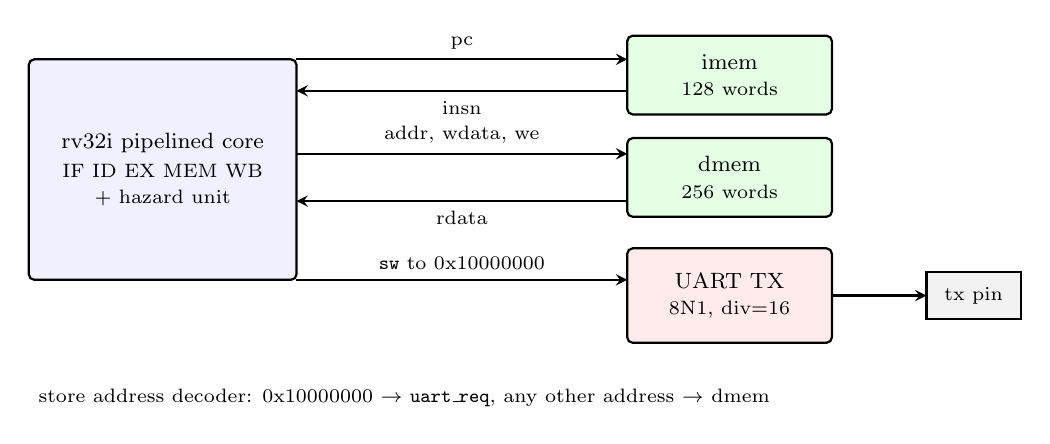
\begin{tikzpicture}[font=\footnotesize, >=stealth, x=1cm, y=1cm]
  \draw[thick, fill=blue!6, rounded corners=2pt] (0,1.0) rectangle (3.4,3.8);
  \node[align=center] at (1.7,2.4) {rv32i pipelined core\\[1pt]
    \scriptsize IF ID EX MEM WB\\ \scriptsize + hazard unit};
  \draw[thick, fill=green!10, rounded corners=2pt] (7.6,3.1) rectangle (10.2,4.1);
  \node[align=center] at (8.9,3.6) {imem\\ \scriptsize 128 words};
  \draw[thick, fill=green!10, rounded corners=2pt] (7.6,1.8) rectangle (10.2,2.8);
  \node[align=center] at (8.9,2.3) {dmem\\ \scriptsize 256 words};
  \draw[thick, fill=red!8, rounded corners=2pt] (7.6,0.2) rectangle (10.2,1.4);
  \node[align=center] at (8.9,0.8) {UART TX\\ \scriptsize 8N1, div=16};
  \draw[thick, fill=gray!10] (11.4,0.5) rectangle (12.6,1.1);
  \node at (12.0,0.8) {\scriptsize tx pin};
  \draw[->, thick] (3.4,3.8) -- node[above]{\scriptsize pc} (7.6,3.8);
  \draw[->, thick] (7.6,3.4) -- node[below]{\scriptsize insn} (3.4,3.4);
  \draw[->, thick] (3.4,2.6) -- node[above]{\scriptsize addr, wdata, we} (7.6,2.6);
  \draw[->, thick] (7.6,2.0) -- node[below]{\scriptsize rdata} (3.4,2.0);
  \draw[->, thick] (3.4,1.0) -- node[above]{\scriptsize \texttt{sw} to 0x10000000} (7.6,1.0);
  \draw[->, thick] (10.2,0.8) -- (11.4,0.8);
  \node[align=left, anchor=west, font=\scriptsize] at (0.0,-0.5)
    {store address decoder: 0x10000000 $\to$ \texttt{uart\_req}, any other address $\to$ dmem};
\end{tikzpicture}
\caption{The ch08 SoC: the pipelined core, instruction memory, data
memory, and a memory-mapped UART. One extra address-compare line
turns an ordinary \texttt{sw} into a serial transmission.}
\label{fig:soc08}
\end{figure}


\section{Minimal traps: \texttt{ecall} and \texttt{mret}}
\label{sec:traps08}

Real RISC-V privilege machinery is large: dozens of control and
status registers, trap delegation, vectored vs.\ direct entry. Two
CSRs carry this chapter:

\begin{itemize}
\item \texttt{mepc}: hardware writes the faulting instruction's pc
      here on trap entry; \texttt{mret} jumps back to
      \texttt{mepc}+4. (Honest caveat: on a real RISC-V core
      \texttt{mret} jumps to \texttt{mepc} itself and the handler
      adds 4 with \texttt{csrr}/\texttt{addi}/\texttt{csrw}. We fold
      that addition into the hardware to keep the demo handler to two
      instructions.)
\item \texttt{mcause}: a small code saying why. Present in our core
      as an extension point --- the demo handler does not read it.
\end{itemize}

The micro-architecture adds three lines to the pc logic: on
\texttt{ecall} in EX, latch \texttt{mepc} and redirect fetch to a
fixed vector (0x80 here); on \texttt{mret}, redirect to
\texttt{mepc}+4; both flush the younger stages like a branch.

\begin{figure}[htbp]
\centering
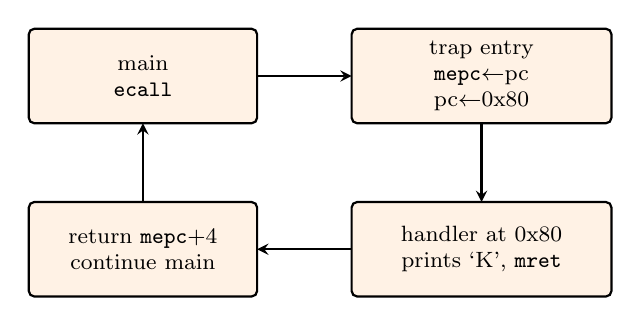
\begin{tikzpicture}[font=\footnotesize, >=stealth, x=1cm, y=1cm]
  \draw[thick, fill=orange!10, rounded corners=2pt] (0,2.6) rectangle (2.9,3.8);
  \node[align=center] at (1.45,3.2) {main\\ \texttt{ecall}};
  \draw[thick, fill=orange!10, rounded corners=2pt] (4.1,2.6) rectangle (7.4,3.8);
  \node[align=center] at (5.75,3.2) {trap entry\\ \texttt{mepc}$\leftarrow$pc\\ pc$\leftarrow$0x80};
  \draw[thick, fill=orange!10, rounded corners=2pt] (4.1,0.4) rectangle (7.4,1.6);
  \node[align=center] at (5.75,1.0) {handler at 0x80\\ prints `K', \texttt{mret}};
  \draw[thick, fill=orange!10, rounded corners=2pt] (0,0.4) rectangle (2.9,1.6);
  \node[align=center] at (1.45,1.0) {return \texttt{mepc}+4\\ continue main};
  \draw[->, thick] (2.9,3.2) -- (4.1,3.2);
  \draw[->, thick] (5.75,2.6) -- (5.75,1.6);
  \draw[->, thick] (4.1,1.0) -- (2.9,1.0);
  \draw[->, thick] (1.45,1.6) -- (1.45,2.6);
\end{tikzpicture}
\caption{The minimal trap path implemented in this chapter's core:
\texttt{ecall} saves the faulting pc in \texttt{mepc} and jumps to the
fixed vector 0x80; \texttt{mret} returns to \texttt{mepc}+4.}
\label{fig:trap08}
\end{figure}


\begin{figure}[htbp]
\centering
\begin{tabular}{llll}
\toprule
CSR & width & written by & read by \\
\midrule
\texttt{mepc}   & 32 & hardware on trap (idex\_pc) & \texttt{mret} \\
\texttt{mcause} & 5  & hardware on trap (code)    & software (full ISA) \\
\bottomrule
\end{tabular}
\caption{The two CSRs this chapter implements. Real RISC-V defines
dozens; two suffice to trap, handle, and return. \texttt{mcause} is
present but unused by the demo --- noted as the extension point for
timer or external interrupts.}
\label{fig:csr08}
\end{figure}


\begin{checkpoint}
Why \texttt{mepc}+4 and not \texttt{mepc}? Because \texttt{mepc}
holds the \emph{ecall's own} address; returning to it would trap
again forever. Real RISC-V handlers choose by editing \texttt{mepc} before
\texttt{mret}: leave it (retry the instruction, as a page-fault
handler does) or add 4 (move on, as a system-call handler does). Our
hardware always adds 4.
\end{checkpoint}

\section{The UART: one shift register with an address}
\label{sec:uart08}

The transmitter is the same 8N1 shape used in the electronics book's
capstone: a 10-bit frame --- start bit, eight data bits least
significant bit first, stop bit --- shifted out at one bit per
\texttt{div} clocks. The only new piece is the request line:

\begin{lstlisting}[language=Verilog,caption={The MMIO hook in
\texttt{rv32i\_soc\_top}: any store word whose address is
0x10000000 becomes a UART transmit request instead of a dmem
write.}]
assign dmem_we  = exmem_memwrite & (exmem_y != 32'h10000000);
assign uart_req = exmem_memwrite & (exmem_y == 32'h10000000);
\end{lstlisting}

\noindent That is the whole of ``device driver'': the store's
address decides where its data goes. Programs use
\texttt{lui a7,0x10000} once and then \texttt{sw tX,0(a7)} for every
byte out.

\begin{figure}[htbp]
\centering
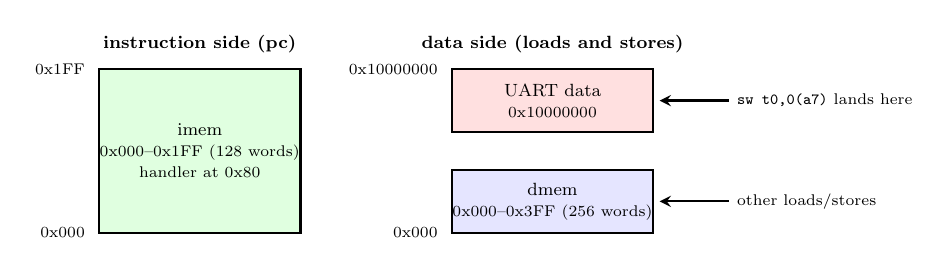
\begin{tikzpicture}[font=\footnotesize, >=stealth, scale=0.8, transform shape]
  % instruction side
  \node[font=\footnotesize\bfseries] at (1.6,6.4) {instruction side (pc)};
  \draw[thick, fill=green!12] (0,3.4) rectangle (3.2,6.0);
  \node[align=center] at (1.6,4.7) {imem\\ \scriptsize 0x000--0x1FF (128 words)\\ \scriptsize handler at 0x80};
  \node[anchor=east, font=\scriptsize] at (-0.1,6.0) {0x1FF};
  \node[anchor=east, font=\scriptsize] at (-0.1,3.4) {0x000};
  % data side
  \node[font=\footnotesize\bfseries] at (7.2,6.4) {data side (loads and stores)};
  \draw[thick, fill=red!12] (5.6,5.0) rectangle (8.8,6.0);
  \node[align=center] at (7.2,5.5) {UART data\\ \scriptsize 0x10000000};
  \draw[thick, fill=blue!10] (5.6,3.4) rectangle (8.8,4.4);
  \node[align=center] at (7.2,3.9) {dmem\\ \scriptsize 0x000--0x3FF (256 words)};
  \node[anchor=east, font=\scriptsize] at (5.5,6.0) {0x10000000};
  \node[anchor=east, font=\scriptsize] at (5.5,3.4) {0x000};
  \draw[->, thick] (10.0,5.5) -- (8.9,5.5) node[pos=0,right]{\scriptsize\texttt{sw t0,0(a7)} lands here};
  \draw[->, thick] (10.0,3.9) -- (8.9,3.9) node[pos=0,right]{\scriptsize other loads/stores};
\end{tikzpicture}
\caption{The two address maps of the ch08 SoC. The core has separate
instruction and data memories (a Harvard layout), each starting at
address 0. Only the data side has a carved-out address,
\texttt{0x10000000}, that belongs to the UART; any other store goes to
\texttt{dmem}.}
\label{fig:mmio08}
\end{figure}


\begin{figure}[htbp]
\centering
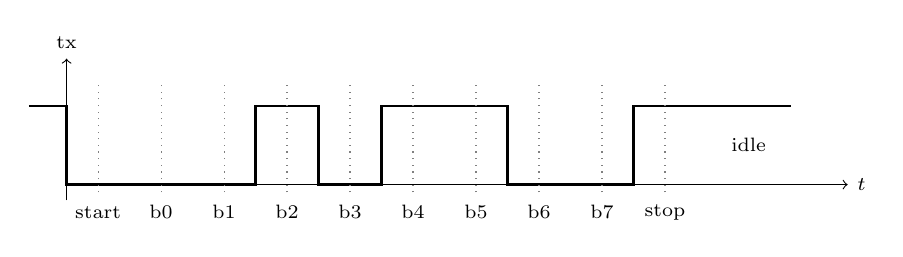
\begin{tikzpicture}[font=\footnotesize, x=8mm, y=10mm]
  % '4' = 0x34 = 0011 0100; 8N1 LSB first: start 0, bits 0,0,1,0,1,1,0,0, stop 1
  \draw[->] (0,0) -- (12.4,0) node[right]{\scriptsize $t$};
  \draw[->] (0,-0.2) -- (0,1.6) node[above]{\scriptsize tx};
  % bit cells: start 0-1, b0 1-2, b1 2-3, b2 3-4, b3 4-5, b4 5-6, b5 6-7, b6 7-8, b7 8-9, stop 9-10
  \draw[thick]
    (-0.6,1) -- (0,1) -- (0,0)   % idle high, falls at start bit
    -- (3,0) -- (3,1)            % start,b0,b1 low; b2 = 1 rises at 3
    -- (4,1) -- (4,0)            % b3 = 0
    -- (5,0) -- (5,1)            % b4 = 1
    -- (7,1) -- (7,0)            % b5 = 1, b6 = 0
    -- (9,0) -- (9,1)            % b7 = 0, stop = 1
    -- (11.5,1);
  \foreach \x/\b/\lbl in {0/0/start, 1/0/b0, 2/0/b1, 3/1/b2, 4/0/b3,
                          5/1/b4, 6/1/b5, 7/0/b6, 8/0/b7, 9/1/stop} {
    \node[font=\scriptsize] at (\x+0.5,-0.35) {\lbl};
    \draw[dotted,gray] (\x+0.5,-0.1) -- (\x+0.5,1.3);
  }
  \node[anchor=west] at (10.4,0.5) {\scriptsize idle};
\end{tikzpicture}
\caption{The wire-level frame the testbench observed for byte
0x34 (ASCII `4'): idle high, one start bit, eight data bits
LSB-first (\texttt{00110100} read right-to-left), one stop bit. Three
falling edges occur inside this one frame (the start bit and the
1-to-0 steps after b2 and b5), which is why a bench that counts
every falling edge on a four-byte message sees 13, not 4.}
\label{fig:uartwave08}
\end{figure}


\begin{example}[Reading the frame]
For byte 0x34 (`4'), the serial line goes low for one bit time
(start), carries \texttt{00110100} LSB-first (so the wire order is
0,0,1,0,1,1,0,0), then returns high (stop). Figure~\ref{fig:uartwave08}
draws the wire; the testbench counts falling edges on \texttt{tx}.
\end{example}

\begin{example}[Counting falling edges: the naive count fails]
A first guess says each frame begins with exactly one falling edge, so
four frames give four edges. Count the real wire instead. The line sits
high while idle, and every 1-to-0 step is a falling edge, whether it
is the start bit or a data bit. Writing each frame as start bit,
\texttt{d0}\ldots\texttt{d7}, stop bit:
\begin{center}
\begin{tabular}{@{}lllc@{}}
\toprule
byte & wire (start, d0..d7, stop) & falls at & count \\
\midrule
0x34 `4' & 0 0 0 1 0 1 1 0 0 1 & start, d2$\to$d3, d5$\to$d6 & 3 \\
0x32 `2' & 0 0 1 0 0 1 1 0 0 1 & start, d1$\to$d2, d5$\to$d6 & 3 \\
0x4B `K' & 0 1 1 0 1 0 0 1 0 1 & start, d1$\to$d2, d3$\to$d4, d6$\to$d7 & 4 \\
0x21 `!' & 0 1 0 0 0 0 1 0 0 1 & start, d0$\to$d1, d5$\to$d6 & 3 \\
\bottomrule
\end{tabular}
\end{center}
\noindent The total is \(3+3+4+3=13\), exactly the number the
testbench printed. (Each frame ends high, so the next start bit is
always a clean 1-to-0 edge.) The ``13 versus 4'' is therefore not a
sign of collisions; it is the data itself. The decoder in the next
section stops guessing and reads the bytes back.
\end{example}

\section{The program, end to end}
\label{sec:program08}

The demo program exercises every door at once. It computes
\(6\times 7\) in a register loop (the same multiply-by-add pattern
from chapter~4), prints the two digits, executes \texttt{ecall},
prints one more character after \texttt{mret}, then parks:

\begin{lstlisting}[language={[x86masm]Assembler},caption={The demo
program (assembled by the book's own assembler into
\texttt{ch08\_prog.hex}). Excerpt --- main loop, UART writes,
\texttt{ecall}, and the handler at 0x80.}]
mloop: add  a2, a2, a0     # a2 += 6, seven times
       addi a1, a1, -1
       bne  a1, zero, mloop
       lui  a7, 0x10000    # UART MMIO base
       li   t0, 52         # '4'
       sw   t0, 0(a7)
       ...delay loop...
       li   t0, 50         # '2'
       sw   t0, 0(a7)
       ecall               # trap: mepc <- pc, pc <- 0x80
       li   t0, 33         # '!'
       sw   t0, 0(a7)
park:  beq  zero, zero, park
# ---- handler at 0x80 ----
       li   t0, 75         # 'K'
       sw   t0, 0(a7)
       mret                # pc <- mepc + 4
\end{lstlisting}

\begin{example}[What the testbench saw]
This is real \texttt{vvp} output, verbatim, from the captured
log \texttt{code/ch08\_soc\_tb.out}:

\begin{verbatim}
ran 770 cyc, pc=00000058, a2=42 (want 42)
MMIO bytes sent: 42K!
uart frames started: 4 (want 4)
tx start-bit edges seen: 13
  ok: 6*7=42 via loop
  ok: '42' to MMIO
  ok: 'K!' trap handler + mret
  ok: serial wire really wiggled
ch08 PASS
\end{verbatim}

Read it slowly. \texttt{42} proves the compute and the data memory.
\texttt{K} proves the trap: the handler ran, did its work, and
\texttt{mret} landed back exactly on the instruction after
\texttt{ecall} --- the \texttt{!}. The line ``tx start-bit edges seen: 13'' is
a trap for the reader: the counter counts \emph{every} falling edge on
\texttt{tx}, and a data bit going from 1 to 0 is a falling edge too.
Thirteen is correct, and the next worked example recounts it by hand.
\end{example}

A counter of edges is weak evidence. A real receiver ignores edges
and does what the standard says: wait for a start bit, sample each
data bit in the \emph{middle} of its time slot, and check the stop
bit. Listing~\ref{lst:wire08} is that receiver written as the second
testbench, \texttt{ch08\_wire\_tb.v}. It never looks inside the CPU to
learn what was sent; it sees only the \texttt{tx} wire.

\begin{lstlisting}[language=Verilog,label={lst:wire08},caption={The wire
decoder (core loop) and its captured output. Run on the book's own
Icarus simulation; \texttt{div}=16 clocks per bit. The cycle numbers
count clocks since reset release.}]
forever begin
  @(negedge tx);                          // start bit begins
  repeat (DIV + DIV/2) @(posedge clk);    // 1.5 bit times: middle of d0
  for (k = 0; k < 8; k = k + 1) begin
    byte_r[k] = tx;                       // LSB first
    repeat (DIV) @(posedge clk);          // next bit's middle
  end
  if (tx !== 1'b1) bad = bad + 1;         // stop bit must be high
  dec[nframes] = byte_r; nframes = nframes + 1;
end

decoded from tx wire: 42K!
frames=4  bad stop bits=0  falling edges on tx=13
  frame 0: byte 0x34  start-bit cycle 42
  frame 1: byte 0x32  start-bit cycle 283
  frame 2: byte 0x4b  start-bit cycle 528
  frame 3: byte 0x21  start-bit cycle 772
ecall in EX at cycle 521; fetch pc becomes 0x80 at cycle 522 (1 cycles later)
mret in EX at cycle 766; fetch pc is back at 0x48 at cycle 767 (1 cycles later)
ch08 WIRE PASS
\end{lstlisting}

\begin{example}[What the wire decoder tells us that the first bench could not]
Three facts. First, the bytes \texttt{0x34 0x32 0x4B 0x21} come off the
wire, not off the bus into the UART: the whole path
store $\to$ transmitter $\to$ pin works, with every stop bit high.
Second, the trap is cheap in cycles but not in work: the core sees
\texttt{ecall} in EX at cycle 521 and the fetch pc is 0x80 one cycle
later; the two instructions fetched behind the \texttt{ecall} are
discarded by the flush. The same one-cycle redirect happens on
\texttt{mret} (cycle 766 $\to$ 767). Third, the gaps between start
bits are 241, 245 and 244 cycles, far longer than the 160 clocks a
frame needs, which prepares the next question.
\end{example}

\begin{example}[How short can the delay loop be?]
The frame needs \(10\times16=160\) clocks, and the UART refuses a new
byte while \texttt{busy}. Each delay iteration is
\texttt{addi} (1 cycle) plus a taken \texttt{bne}, which flushes two
younger instructions (2 cycles): about 4 cycles per iteration. The
naive estimate is \(160/4=40\) iterations. Test it rather than trust
it: rewrite the constant \texttt{li t1,60} to \texttt{li t1,}\(N\) in
the hex file and rerun the decoder (the test script does this). Captured:

\begin{verbatim}
delay sweep: N=39 -> 2 frames, N=40 -> 4 frames
\end{verbatim}

At \(N=39\) the second byte (`2') is silently lost and only `4' and
`K' arrive; at \(N=40\) all four arrive, with the first gap at 161
cycles, i.e.\ \(4N+1\). The sweep confirms the estimate to the cycle,
and shows what ``dropped, not queued'' looks like: no error, just a
missing character. With \(N=60\) the program has a margin of 80
cycles, and the three delay loops account for about
\(3\times240=720\) of the first 772 cycles of the run.
\end{example}

\begin{checkpoint}
Why do consecutive \texttt{sw}s to the UART need a delay loop between
them? The transmitter is busy for \texttt{div}$\times$10 clocks;
a store arriving mid-frame has nowhere to queue. Real chips answer
with a status bit the software polls --- our minimal UART teaches
the collision honestly instead.
\end{checkpoint}

\section{Receipts: two bugs this chapter paid for itself}
\label{sec:receipts08}

\begin{example}[The WB/ID boundary hazard --- a fourth hazard class]
Chapter~7 claimed data, control, and structural hazards covered
everything. The trap program exposed a fourth: a writer leaving the
pipeline at WB on the same edge a reader latches its operands in ID.
The regfile read \texttt{a1 = 0} one cycle too early, the
\texttt{addi a1,a1,-1} computed \(-1\) instead of \(6\), and the loop
ran 4\,038 times instead of 7. Fix, and the classic textbook answer:
a write-bypass \emph{inside} the register file so a WB write is
visible to a concurrent ID read (``write first''). One line each on
\texttt{rd1}/\texttt{rd2} --- and it removed the hazard for every
program, not just this one.
\end{example}

\begin{example}[The trap vector pointing at a data table]
The first run of the new core went to 0x40 on \texttt{ecall} ---
because the handler had been placed at byte 0x80 while
\texttt{MTVEC} still said 0x40. The machine faithfully trapped
into the middle of its own main program (executing a \texttt{bne}
as if it were handler code) and never came back. The debugger showed
\texttt{pc} frozen at 0x44 --- the \texttt{ecall}'s own address,
re-trapped on every return because \texttt{mret} landed back on it.
Two-line fix (0x40$\to$0x80), and a permanent lesson: a trap
vector is an address like any other; getting it wrong produces the
most confusing bug in the book --- a processor that is \emph{correct}
about everything except where it jumps.
\end{example}

\section{What it costs in silicon}
\label{sec:synth08}

\begin{figure}[htbp]
\centering
\begin{tabular}{lr}
\toprule
cell class & count (real \texttt{synth\_gowin} run) \\
\midrule
LUT1--LUT4           & 2\,021 \\
MUX2\_LUT5--LUT8     & 1\,103 \\
ALU (fast carry)     & 186 \\
DFF variants         & 527 \\
RAM16SDP4            & 32 \\
IO buffers           & 166 \\
\midrule
\textbf{total}       & $\approx$4\,035 \\
\bottomrule
\end{tabular}
\caption{Real \texttt{yosys-0.69 synth\_gowin} output for the whole
SoC (core + UART + trap CSRs). The GW1NR-LV9 offers 8\,640 LUT4 ---
this machine plus its peripherals uses about half. The 32
RAM16SDP4 blocks are the register file inferred as LUT-RAM.}
\label{fig:synth08}
\end{figure}


The whole machine --- 5-stage pipelined RV32I core with forwarding,
stall, flush, trap CSRs, plus the UART --- synthesises to roughly
4\,000 cells on the GW1NR-LV9, about half its LUT budget. Compare
with the 302-cell \texttt{cpu8} from the electronics book: the
pipelining machinery costs an order of magnitude more logic, and buys
the order of magnitude in clock rate back.

\section{Common mistakes}
\label{sec:mistakes08}

\begin{itemize}
\item \textbf{MMIO store eaten by silence.} A store to
      0x10000000 while \texttt{busy} is high is dropped, not
      queued. Check a status bit, or pace the writes.
\item \textbf{\texttt{mret} to \texttt{mepc}, not \texttt{mepc}+4.}
      Re-executes \texttt{ecall}: an infinite trap loop that looks,
      in a wave viewer, like a machine ``stuck'' at one address.
\item \textbf{Trap vector overlapping program code.} If the handler
      region is not reserved, the trap entry jumps into the middle
      of normal code --- the machine does nonsense very competently.
\item \textbf{Forgetting that flush kills the trap's own fetch.} The
      redirect takes effect on the \emph{next} fetch; the
      instructions already in flight must be bubbled, or the handler
      interleaves with dying main-code instructions.
\item \textbf{Assuming the regfile boundary is free.} WB and ID
      touch the same storage on the same edge; without an explicit
      ordering (write-bypass, or write-first timing) it is a
      data hazard that stalls cannot fix.
\end{itemize}

\section*{Further reading}
\label{sec:fr08}
\begin{itemize}
\item Patterson \& Hennessy, \emph{Computer Organization and
      Design}, RISC-V edition --- sections on exceptions and
      memory-mapped IO (the canonical treatment this chapter follows).
\item Harris \& Harris, \emph{Digital Design and Computer
      Architecture, RISC-V ed.} --- the pipelined-processor chapter;
      our core is a small honest version of theirs.
\item The RISC-V Instruction Set Manual, Volume~II: Privileged
      Architecture --- \texttt{mepc}, \texttt{mcause},
      \texttt{mtvec} definitions we shrink to two registers.
\item Ben Eater's video documentation of his 8-bit computer's output
      register --- the same MMIO idea on a breadboard machine
      (the Book~5 capstone's ancestor).
\end{itemize}

\begin{rulebox}[Watch instead]
\begin{itemize}
\item \textbf{Exceptions \& Interrupts} --- Computerphile
      (YouTube, verified 2026-10-11): why traps exist at all, at the
      right altitude for this chapter.
      \url{https://youtu.be/FR4rmlkgwr4}
\item \textbf{8-bit computer output register} --- Ben Eater
      (YouTube, verified 2026-10-11): the memory-mapped output idea
      on a real breadboard machine; the direct ancestor of our UART
      hook. \url{https://youtu.be/9Ma3c8xZJk8}
\end{itemize}
\end{rulebox}

\section*{Notes}
\label{sec:notes08}
\begin{itemize}
\item Trap semantics follow the RISC-V privileged spec reduced to
      two CSRs; the UART is the Book~5 capstone serialiser unchanged.
\item All outputs are verbatim Icarus runs of the chapter's
      testbench; both bug receipts in sec:receipts08 are real
      session bugs, fixed in-tree.
\end{itemize}

\section{Summary}
\label{sec:summary08}
\begin{tabularx}{\linewidth}{@{}l X@{}}
\toprule
\textbf{Piece} & \textbf{What this chapter added} \\
\midrule
Trap entry  & \texttt{ecall}: \texttt{mepc}$\leftarrow$pc, pc$\leftarrow$0x80, flush \\
Trap return & \texttt{mret}: pc$\leftarrow$\texttt{mepc}+4, flush \\
MMIO        & address-compare turns \texttt{sw} into a device request \\
UART        & 8N1 shift register, \texttt{busy} honest about collisions \\
Regfile     & write-bypass: the fourth (WB/ID) hazard, fixed once \\
Program     & \texttt{42K!} on a decoded wire: compute, IO, trap, return \\
Cost        & $\approx$4k cells: pipelining bought speed at 10$\times$ logic \\
\bottomrule
\end{tabularx}

% ------- exercises -------
\section*{Exercises}
\addcontentsline{toc}{section}{Exercises}
\stepcounter{section}

\begin{exercise}[easy]

Write the two RV32I instructions a program needs to send byte
0x41 (`A') to the UART, given that the base register already
holds 0x10000000. What happens if the instruction immediately
before it was also a UART store?
\end{exercise}
\begin{solution}[hint]
One \texttt{li} plus one \texttt{sw}; the previous frame must
have finished or the write is dropped.
\end{solution}

\begin{exercise}[easy]

\texttt{mepc} currently stores the \texttt{ecall}'s address. What
would you change if the handler needed to distinguish an
\texttt{ecall} from an illegal instruction? Which CSR, which value?
\end{exercise}
\begin{solution}[hint]
\texttt{mcause} exists but is never written a distinct code;
assign one per trap source.
\end{solution}

\begin{exercise}[easy]

Why does the trap-entry logic live in EX rather than ID in this
core? What would break if it redirected the pc while the offending
instruction was still in ID?
\end{exercise}
\begin{solution}[hint]
Younger stages still carry the pre-trap instruction stream;
the redirect must coincide with the flush.
\end{solution}

\begin{exercise}[easy]

The UART has no receive side. Which two wires/registers would a
receiver need that the transmitter does not have?
\end{exercise}
\begin{solution}[hint]
A sampling clock at the bit rate and a byte-valid flag ---
plus somewhere to buffer the byte.
\end{solution}

\begin{exercise}[medium]

Our handler is at a fixed address. Sketch the pc-mux change for a
\emph{vectored} trap where \texttt{mcause} selects among four
handler addresses. Which existing block does most of the work?
\end{exercise}
\begin{solution}[hint]
It is the same mux \texttt{jal}/branch already use --- one
more input.
\end{solution}

\begin{exercise}[medium]

Using the wire decoder's numbers (ecall in EX at cycle 521, fetch pc
equal to 0x80 at cycle 522), how many cycles after the \texttt{ecall}
reaches EX is the first handler instruction \emph{fetched}? Then,
counting pipeline stages, in which cycle does it reach EX? Which
stage sets the floor on trap latency?
\end{exercise}
\begin{solution}[hint]
Fetched one cycle later (522). From IF it needs ID then EX, so it
reaches EX two cycles after that, in cycle 524. The floor is where the
redirect is decided: EX, three stages behind fetch.
\end{solution}

\begin{exercise}[medium]

Add a second MMIO device: a byte-wide output latch at
0x10000004 driving eight LEDs. How many Verilog lines change?
What class of bug appears if two MMIO addresses alias by accident?
\end{exercise}
\begin{solution}[hint]
One more address compare; aliased ranges write both devices.
\end{solution}

\begin{exercise}[medium]

The demo pads UART writes with a software delay loop. Design the
polling version instead: a read of 0x10000004 returns
\texttt{busy}. Which datapath piece must grow to support an MMIO
\emph{read}?
\end{exercise}
\begin{solution}[hint]
The load mux --- reads need a mux input just like stores need
an address compare.
\end{solution}

\begin{exercise}[hard]

Argue for or against: on a real RV32I, the trap-entry redirect
should also record \texttt{mtval} (the faulting address/instruction).
What goes wrong in our design without it, for a handler that wants
to emulate the trapped instruction?
\end{exercise}
\begin{solution}[hint]
Without the instruction bits or the bad address, emulation has
nothing to emulate; the handler must decode \texttt{mepc}'s target
itself --- possible, but doubles the work.
\end{solution}

\begin{exercise}[hard]

We fixed the WB/ID hazard with a register-file bypass. An
alternative is to write the regfile on the negedge of the clock.
Compare the two: which buys the fix more cheaply, and which survives
a timing-closed synthesis better? Defend a choice.
\end{exercise}
\begin{solution}[hint]
Negedge writes halve the regfile's setup slack; the bypass is
two muxes but keeps everything single-edge.
\end{solution}

\begin{exercise}[hard]

Estimate the share of the demo program's cycles spent in its three
delay loops (60 iterations each), using the measured run: the last
start bit appears at cycle 772. What is the loops' CPI? How would a
busy-poll loop change the accounting?
\end{exercise}
\begin{solution}[hint]
Each iteration retires 2 instructions (\texttt{addi}, \texttt{bne}) in
about 4 cycles, so CPI $\approx 2$. Three loops give
$3\times60\times4=720$ cycles, about $720/772\approx 93\%$ of the
run. A busy-poll loop spins on a load plus a branch, also costing a few
cycles per poll, but it exits the moment \texttt{busy} clears instead
of waiting out a fixed worst case.
\end{solution}

\begin{exercise}[hard]

The core has no interrupt line --- nothing can trap it from outside.
Describe the minimal external interrupt mechanism (one pin, one
pending bit) and where in the pipeline you would sample it. Why is
``sample between instructions'' easier said than done?
\end{exercise}
\begin{solution}[hint]
You need a point where the pipeline drains cleanly; sampling
in EX like \texttt{ecall} works if the pin is level-sensitive and
the handler disables re-entry.
\end{solution}

\begin{exercise}[easy]
The testbench runs the UART with \texttt{div}=16. If the same design
were clocked at 27\,MHz with \texttt{div}=16, how many clocks does one
8N1 frame take, what is the baud rate, and how many bytes per second can
be sent at most?
\end{exercise}
\begin{solution}[hint]
A frame is 10 bits of 16 clocks each.
Frame $=10\times16=160$ clocks. Baud $=27\,000\,000/16=1\,687\,500$
bits per second. Bytes per second $=27\,000\,000/160=168\,750$.
\end{solution}

\begin{exercise}[medium]
Write the wire order (start bit, d0 to d7, stop bit) of the byte 0x41
(`A') and count the falling edges the decoder's edge counter would add
for it, starting from an idle-high line.
\end{exercise}
\begin{solution}[hint]
$0x41=01000001$; send d0 first.
Wire: 0 | 1 0 0 0 0 0 1 0 | 1. The 1-to-0 steps are the start bit,
d0$\to$d1 and d6$\to$d7: 3 falling edges.
\end{solution}

\begin{exercise}[medium]
Reading the sweep: at \(N=40\) the gap between the first two start
bits was 161 cycles, and at \(N=60\) it was 241. Fit the model
gap\,$=aN+c$ to these two points, then predict the gap for \(N=50\)
and say whether `2' survives.
\end{exercise}
\begin{solution}[hint]
Two points give the slope: $(241-161)/(60-40)=4$ cycles per iteration,
so $c=161-4\cdot40=1$. Then gap$(50)=201$. A frame needs $\approx161$
cycles from the store, so 201 is safe: all four bytes arrive.
\end{solution}
